%!TEX root = ../dissertation.tex

\chapter{State-Of-The-Art}
\label{chapter:state_art}
In this chapter, Data Streaming and Vector Extension will be discussed through the presentation of some of the state-of-the-art implementations of these technologies.


%There has been a growing demand for faster General-Purpose Processors (GPPs) which has led to a lot of development in improving the speed of instruction execution and overall clock speed. However as the usage of data-intensive programs like machine learning and artificial intelligence continues to grow, it is becoming increasingly clear that enhancing the processor speed alone will not be sufficient if they depend heavily on surrounding components such as memory. 

%To tackle this issue, various techniques have been developed and studied in the field of memory reading and writing as well as data manipulation. These methods include data-level parallelism, memory access prefetching, memory caching, data streaming, and others.


\section{Data Streaming}
Specializing the core computation part of a processor and relying only on traditional memory abstractions is not sufficient for the necessary improvements on modern-day CPUs \cite{8192490}. As a matter of fact an area where specialization has not advanced at the same pace as other components is memory primitives. Exposure to more memory information at the ISA level and utilizing unique micro-architecture mechanics would allow for tackling multiple shortcomings with memory use in the core. Some of these shortcomings are the added overhead in the pipeline on data indexing and memory address generation, the overlapping memory requests, and transfers from the memory system.

The solution for some of these problems might lie in using dedicated structures of memory access such as data streams \cite{8192490}. Data streams are easily constructed through the analysis of repeated patterns of memory accesses, most of the time associated with loops and nested loops of programs.

The following subsections present a brief overview of some recent state-of-the-art proposals to address data streaming in accelerators and general purpose processors.


\subsection{Stream Accelerators for Data Manipulation}
\label{label:stream_dataflow}
Stream Dataflow denotes an implementation of an accelerator proposed by Nowatzki \textit{et al.} \cite{8192490} with the sole purpose of managing streamed memory accesses. According to its authors, the proposed architecture can serve as the basis of configurable memory accelerators.

The acceleration unit proposed in this project was designed with the objective of achieving as good of performance as an application or domain-specific system while trying to maintain efficiency and utilization abstraction. The approach taken to achieve such goals was through the use of data stream memory structures.

\begin{figure}[H]
	\begin{center}
 		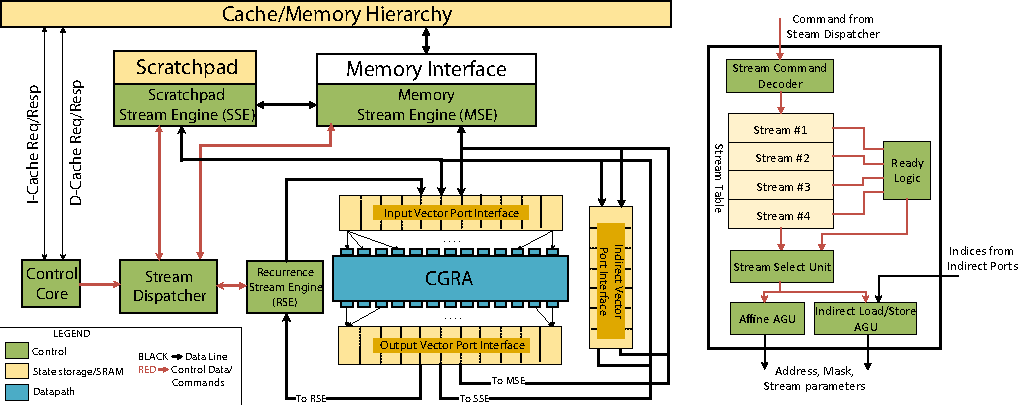
\includegraphics[width=0.87\linewidth]{images/stream-dataflow arch.pdf}
 		\caption{Stream Data Flow micro-architecture (Softbrain) (left); Stream engine pipeline (right) - Figure from \cite{8192490}}
 		\label{fig:stream-dataflow_arch}
	\end{center} 
\end{figure}

The proposed micro-architecture, called \textit{Softbrain}, can be seen in Figure \ref{fig:stream-dataflow_arch} (Left), and it is composed of five primary components:

\begin{itemize}
    \item \textbf{Control Core} - Tasked with the generation of stream-dataflow commands;
    \item \textbf{Stream Dispatcher} - Unit that tracks stream resource dependencies, issues commands to stream engines, and manages concurrent stream execution.
    \item \textbf{Stream Engines} - 3 engines that carry out the data access: one for memory (facilitating wide access to memory), one for scratchpad (efficient data reuse), and one for DFG recurrences (for immediate reuse). The use of each engine is dependent on the streams that are assigned to them.
    \item \textbf{Vector Ports} - The main interface between the computation that is carried out in the CGRA and the streams. A set of isolated vector ports allows for indirect memory loads/stores.
    \item \textbf{Main Acceleration Unit (CGRA)} - The coarse grained reconfigurable pipeline where the main processing of the dataflow graphs is conducted. 
\end{itemize}

The Stream-Dataflow accelerator operates by executing precompiled graphs known as DataFlow Graphs (DFG). The compilation of these graphs occurs alongside program compilation and consists of multiple instructions organized in a network of operations and dependencies. 


During runtime, the main acceleration unit is reconfigured according to the DFG to correctly map the input and output of the vector ports and define the appropriate vector length for compatibility with the memory streams. Additionally, this functional unit is set up for the operations specified by the flow of the graph, creating the advantage of smooth execution of the operations without the need for control inside the CGRA unit.


\subsubsection{Streams}

The stream data structures utilized in the Dataflow Graph Accelerator are defined by 3 parameters: a source location, a destination, and an access pattern. Both the source and destination are associated with a memory address, programmable scratchpads, or a named vector port.

Port locations are associated with the CGRA unit, making the associated streams serve as inputs and outputs of the DFG. 

DFG ports support simple first-in-first-out patterns, while memory and scratchpad access patterns can be more intricate, incorporating features such as strides, repetitions, indirect access, scatter-gather, etc.

Streams typically operate concurrently, but those associated with the same DFG port must execute sequentially.


\subsubsection{Streaming Engines}
In order to be able to utilize stream data structures and take advantage of the high parallelism and low power overheads \cite{8192490}, streaming engines need to be implemented into the micro-architecture. The proposed design for each of the two implemented engines is driven from the diagram illustrated in Figure \ref{fig:stream-dataflow_arch} (Right) and works as a pipeline system.


The engine operates by decoding instructions issued by the dispatcher, keeping track of the number of active streams, and maintaining associated data for each stream. On each clock cycle, the engine selects one of the active streams and generates the required address and data transfer commands. Additionally, it monitors backpressure signals to ascertain if a stream is considered ready. This readiness condition implies that the destination port is not full, and data can be fetched from the source.

As was referred before, the memory system comprises two engines: the memory stream and the scratchpad stream. The memory stream engine is tasked with facilitating the transfer of data to and from the primary memory cache, utilizing streams, and incorporating memory buffering. On the other hand, the scratchpad stream engine bears resemblance to the memory stream engine. However, it is distinct in that it features its dedicated ported SRAM, supporting single-read and single-write operations. 


\subsubsection{Stream-Dataflow ISA}
For the correct operation of the stream-dataflow micro-architecture, three main types of instructions were defined:
\begin{itemize}
    \item[] \Tbullet{T1}{DFG Specification} Given that the physical architecture may impose limitations on the number of instructions for each type in a graph, several constraints on the size of the input and output vectors, and the number of inputs and outputs, the configuration of such parameters could become cumbersome. For that reason, Nowatzki \textit{et al.} \cite{8192490} have chosen to simplify the matter by introducing a single instruction that loads a compiled configuration directly from memory.
    
    \item[] \Tbullet{T2}{Stream Specification} The provided instructions enable the configuration of streams for access with various patterns. These instructions are versatile and can be set up for the most common type of memory access pattern, namely, two-dimensional affine accesses. The definition of such patterns involves specifying the access size, the stride value (size between consecutive accesses), and the number of strides. Additionally, indirect streams can be configured by designating one stream's output as input for another stream.
    
    \item[] \Tbullet{T3}{Barrier Specification} The proposed \acrfull{ISA} includes three barrier instructions. Two of them synchronize the reading and writing of the scratchpad memory, while the third ensures the completion of the \acrfull{DFG} and guarantees that the correct data is stored in the host memory.
\end{itemize}

\subsubsection{Result Analysys}

To assess the goal of designing an accelerator that could replace a domain-specific implementation while maintaining generality, Nowatzki \textit{et al.} \cite{8192490} conducted a series of workload tests from the MachSuite. Each test was run by a \textit{Softbrain} implementation, configured to a max of 20 DFG instructions, and a customized Aladdin ASIC with its implementation generated for each application. %The choosing of the ASIC Design for each test was done through the analysis of multiple implementations in order to find the one closest to the \textit{Softbrain} performance while minimizing power, area, and execution time.
The comparison focused on their power consumption, performance, energy efficiency, and area.

Both the Softbrain and the ASIC implementations showed 1-7x speedup gains across all workloads when compared with a SandyBridge OOO Quad-Core, keeping on par with one another. In terms of power and energy efficiency, the \textit{Softbrain} accelerator showed worse results than the ASICs implementations, however not far behind it. 

On area comparison, the \textit{Softbrain} showed a bigger area use however, since \textit{Softbrain} is programmable on runtime and able to run all workloads, it is possible to advocate that the \textit{Softbrain} implementation is more area efficient than the ASIC implementation since designing a system for the full set of benchmarks performed would require 2.4x the area of \textit{Softbrain}.

Nowatzki \textit{et al.} \cite{8192490} conclude by stating that the developed work demonstrates the potential of designing programmable/configurable architecture that leverage the advantages of streaming structures.


\subsection{Stream-based Memory Access Specialization for General Purpose Processors}

In a follow-up research to the work developed by Nowatzki \textit{et al.} in Stream-Dataflow Acceleration\cite{8192490}, Wang and Nowatzki (2019) \cite{8980305} set out to apply some other same streaming principles on General Purpose Out-of-Order Processors, with the main objective of enhancing the data fetching capabilities of such systems.

Through the use of stream-decoupling, prefetching, and specialized cache policies, the authors aim to reduce the instruction pressure on the processor's pipeline while also making the delivery of data to the processor faster.

\subsubsection{Microachiteture Extension}
In order to keep modifications to the existing microarchitecture to a minimum, most of the frontend structure of the core was maintained unaltered, with the exception of the addition of an iteration map, that tracks the position of each stream index by mapping it to a counter table, the introduction of FIFOs that store the accessed data of the streams, and the implementation of a streaming engine. The location of these units is shown on the left side of Figure \ref{fig:SD_architeture}.

\begin{figure}[H]
\begin{center}
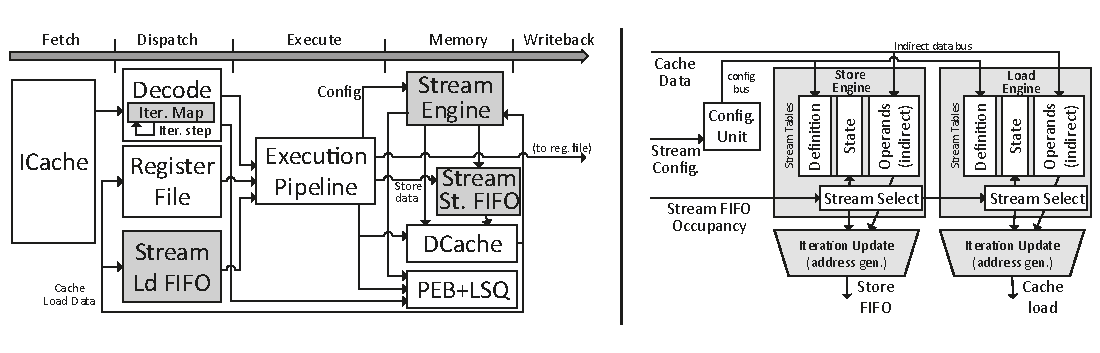
\includegraphics[width=0.87\linewidth]{images/SD_architeture.pdf}
\caption{Stream Specialized Pipeline (Left); Stream Engine (Right) - Figure adapted from \cite{8980305}}
\label{fig:SD_architeture}
\end{center}
\end{figure}


The streaming engine comprises two identical units, one designated for loading from memory and the other for storing in memory. These units incorporate a set of tables employed to describe the state of any configured stream. The \textbf{definition table }encompasses the pattern (affine, indirect, linked) along with the parameters of the access (stride, width, size). The second table is the \textbf{state table }, responsible for storing the memory view of the induction variables, indicating the current address. Lastly, the \textbf{operands table }contains information on any stream dependencies.
Through the use of this stored information, the streaming engine generates, on each clock cycle, the memory address of the following reads/stores caused by the execution pipeline.

The FIFOs of the streaming engine have the purpose of holding the decoupled state either for storing or loading. Whenever a core instruction makes a read to a stream, it accesses the data on the load FIFO. Whenever a core instruction performs a store, the value to store is combined with a previously generated address kept in the store FIFO.


\subsubsection{Decoupled-Stream ISA}

The stream-specialized interface proposed by Wang and Nowatzki (2019) \cite{8980305}, tries to maintain the stream data structure implementation separated from the rest of the cores' microarchitecture maintaining a higher level of abstraction. This is made through the use of special pseudo-registers to which the execution pipeline has access and are mapped to specific data streams. The streaming part of the system applies a similar principle to the Stream Dataflow Accelerator in the sense that it is configurable through an initial instruction.

The execution of code compiled for this stream interface contains such instruction at the beginning of code sections that will benefit from data streaming (loop portions of code). It is responsible for: \textbf{setting up} the necessary \textbf{pseudo-registers} employed by the core pipeline and mapped to the \textbf{data streams}, configuring the \textbf{streams type} (induction/memory) and \textbf{pattern} (stride, width, and optional length),  the dependencies and the starting address. The configuration of streams can also be made to address another stream, thereby establishing a dependency through indirect memory access.

During the execution of the code in the pipeline, a "step" instruction is employed to advance the position of the stream by modifying the induction variables related to the streams and providing the core with abstract information on the stream's progress. At the end of the loop iterations, the configured streams are deallocated and released for the next utilization.

The proposed Instruction Set Architecture (\acrshort{ISA}) incorporates a set of instructions that enable fundamental stream operations, like pattern definitions and data width configuration, supporting complex accesses to data and coalescing of data structures. 

Figure \ref{fig:SD_execution} depicts four examples of the decoupled-stream pseudo-code, along with its stream dependence graph.

\begin{figure}[H]
\begin{center}
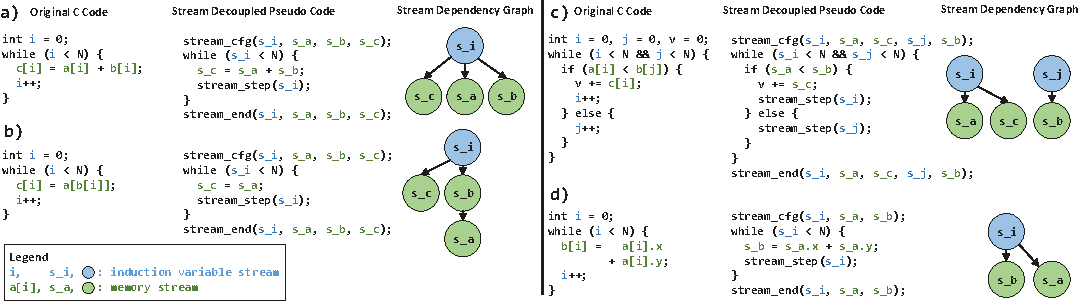
\includegraphics[width=0.97\linewidth]{images/SD_execution.pdf}
\caption{Pseudo Code Examples - Figure adapted from \cite{8980305}}
\label{fig:SD_execution}
\end{center}
\end{figure}

\textbf{\textit{stream\_cfg}} is the instruction used for the configuration, defining all the streams within the loop. After configuration, the stream engine can start fetching data based on the knowledge previously defined.

The use of \textbf{\textit{stream\_step}} inside loop iterations advance the induction variable stream, altering the stream pseudo-register position and resulting in a cascade on all dependent streams. This behavior is evident in the Stream Dependency Graph, where the advancement of \textit{s\_i} causes all dependent streams (\textit{s\_a, s\_b, s\_c, ...}) also to advance.

The \textbf{\textit{stream\_end}} instruction, as the name implies, the utilization of streams concludes by deallocating and releasing the mapped pseudo-registers.

The proposed \acrshort{ISA} comes with its limitations since the decoupling nature of the implementations becomes limited whenever the access patterns cannot be determined at the configuration step. Such cases are conditionally used data and unknown length for an access pattern.


\subsubsection{Using Stream Information}
Wang and Nowatzki (2019) \cite{8980305} also propose the exploitation of the stream information provided by the decoupled design of the presented implementation. Accordingly a prefetching technique and stream-aware cache bypass policies were implemented leveraging such stream information.

In what concerns the prefetching, the distance in which prefetching is made can highly impact the smooth operation of a cores' pipeline. In an ideal prefetcher, the required data would be provided whenever the corresponding load instruction is ready to be issued. This means that a sign of poor performance of the prefetcher could be falling behind on the data requests. For the monitoring and correct utilization of the resources of the processor, Wang and Nowatzki (2019) \cite{8980305} took the approach of implementing a set of counters that track the number of stalls that occur with each stream pseudo-register, entitling it as the dynamic throttling prefetching system. These counters enable the pipeline to dynamically readjust the size distribution of the Load FIFO across stream pseudo-registers. This adjustment provides streams with increased available space and subsequently allow the prefetching distance of specific streams to be incremented based on the rate at which data is being consumed.

In the proposed implementation, the initial value of each stream pseudo-register length is defined in the configuration step with a default value. However, this could be further improved by defining a more personalized value during compilation.

Another technique implemented by Wang and Nowatzki (2019) \cite{8980305} that leverages the information given by the patterns defined by streams, is cache bypassing. In memory requests with low temporal locality, the utilization of cache can become a problem and hurt the overall execution performance. Through the stream information provided by the system (memory footprint, stream length, reuse distance etc), it is possible to decide whether a memory request should be made to the cache or bypass it completely and request the information directly to the memory system. This technique would help avoid polluting the cache with data that would not be reused, as well as avoid unnecessary time wasted with tag lookup and MSHR allocation.


\subsubsection{Result Analysis}

Wang and Nowatzki (2019) \cite{8980305} concluded through a series of workloads that their proposed decoupled-stream ISA extension show very promising results in terms of performance and energy consumption when compared with the baseline simulated 8-Way OOO processor. The tests conducted were made to evaluate the impact of the improvements suggested by the authors, like the inclusion of streaming with prefetching, the utilization of a dynamic throttle of the prefetching distance, and the utilization of stream access information in cache bypassing policies.

The implementation of just the streaming engine resulted in an overall gain of 1.20x in performance. Utilizing both the dynamic throttle (prefetching stall counters) and stream-aware cache policies pushed the gain value to 1.67x when compared with the baseline out-of-order core. In terms of energy efficiency, the implementation of the proposed full system resulted in an improvement of 1.53x compared to the baseline.

Wang and Nowatzki (2019) \cite{8980305} concluded that utilizing the benefits of stream-based prefetching, address computation decoupling, and stream-aware cache policies can lead to a faster, more specialized access and communication within the cache and memory hierarchy, albeit with certain limitations like the problem of unknown length of patterns during stream configuration.

Some further research topics like vector data manipulation could also be seen as a possible improvement to the described system leveraging parallel computation of data.

\subsection{Stream Semantic Registers}
\label{label:ssr}

Stream Semantic Registers (SSR) \cite{9068465} introduces an innovative approach to address the von Neumann bottleneck in single-issue processor cores. This bottleneck arises from the explicit fetch and issue of load/store instructions for data to reach the Arithmetic Logic Units (ALUs) and Functional Units (FUs). In order to mitigate this bottleneck, Schuiki \textit{et al.} \cite{9068465} presents a solution in the form of a straightforward and lightweight RISC-V ISA extension. This extension implicitly encodes memory accesses, thereby reducing the number of instructions associated with memory accesses and enhancing the overall energy efficiency of the system.

To enable this capability, SSR gives some registers stream semantics, meaning that reading from or writing to such registers triggers a direct read or write operation in the memory. This innovative approach streamlines the execution of instructions and contributes to energy efficiency.

\subsubsection{Micro-achiteture}

The following modifications to the processor's core are necessary to implement the SSR system, and allow the mapping of register access to the stream interfaces:

\begin{itemize}
\item[] \Tbullet{C1}{Register File Extension:} Expanding the register file to facilitate the interception and rerouting of accesses to a subset of registers.
\item[] \Tbullet{C2}{Stream Interfaces:} Incorporating stream interfaces to each register file port to allow stream semantics registers.
\item[] \Tbullet{C3}{Control:} Implementing a Control and Status Registers (CSR) to enable or disable stream semantics.
\item[] \Tbullet{C4}{Data Paths:} Adding the paths needed for the communication of stall conditions and back-pressure path to the core's main controller.
\end{itemize}

Schuiki \textit{et al.} \cite{9068465} designed the needed modifications with the added intent of minimizing the impact on the complexity of the underlying architecture. A high-level schematic of the architectural changes needed for this implementation can be seen in Figure. \ref{fig:ssr-overview}.

\begin{figure}[H]
	\begin{center}
 		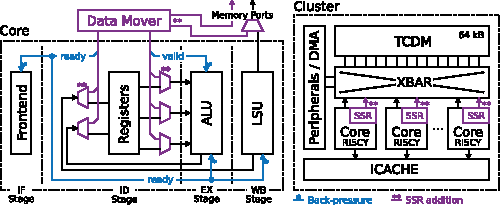
\includegraphics[width=0.87\linewidth]{images/ssr-overview.pdf}
 		\caption{High-level data flow of the SSR extension in a single core  - Figure from \cite{9068465}}
 		\label{fig:ssr-overview}
	\end{center} 
\end{figure}

\subsubsection{Register Files}

The primary architectural modification introduced by the SSR extension is in the processor register file. This register file is structured as a default three read and two write port configuration. However, each port is customized to incorporate the needed circuitry (refer to Fig. \ref{fig:ssr-stream_enable_check}) to intercept read/write accesses and detect whether the specified register has stream semantics enabled.

The process of a register access unfolds as follows: the access is intercepted, the presence of stream semantics is determined, and if confirmed, the access is rerouted to the respective external stream interface connected to the data mover unit.

\begin{figure}[H]
	\begin{center}
 		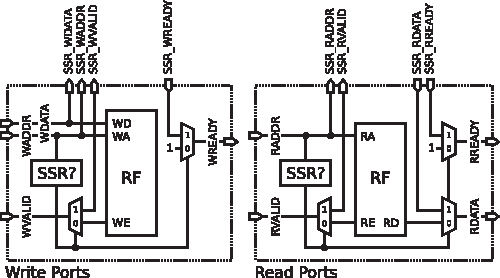
\includegraphics[width=0.67\linewidth]{images/ssr-circuitry.pdf}
 		\caption{Required circuits for stream semantic enabled verification  - Figure from \cite{9068465}}
 		\label{fig:ssr-stream_enable_check}
	\end{center} 
\end{figure}

The confirmation of the active status of stream semantics is carried out in the \textit{SSR} section of the circuit, as illustrated in Fig. \ref{fig:ssr-stream_enable_check}. This verification involves checking the following conditions:

\begin{itemize}
\item[1] The register address connected to the WADDR or the RADDR must correspond to one of the registers allowed to utilize stream semantics, on the write ports circuit or read ports circuit, respectively;
\item[2] The stream semantics flag must be enabled in the core's CSR;
\end{itemize}

In case both conditions are true then the transaction is routed out of the core through a stream interface to the data mover.

\subsubsection{Data Mover}

The accesses initiated within the core and directed outward through the stream interfaces reach the data mover unit. This segment of the architecture, visible in Figure \ref{fig:ssr-data_mover} is tasked with accurately mapping the incoming accesses to the memory system. To execute this function, the data mover incorporates a set of lanes, each comprising a \textit{First-In-First-Out (FIFO)} queue buffer and an address generator unit (AGU). The AGU is responsible for associating each streamed access with the corresponding memory address, whether for reading or writing. Offloading the memory address generation outside of the main pipeline reduces the pressure caused by this type of function.

The internal diagram of the AGU can be seen on the right of Figure \ref{fig:ssr-data_mover} and is based on AGU presented by Schuiki \textit{et al.} \cite{8502059}. It works through the configuration of the hardware loops ($L0$ to $L3$), which are composed of 16-bit counters that iterate over the parameters of the stream access pattern and provide the values necessary for the address generation. 

\begin{figure}[H]
	\begin{center}
 		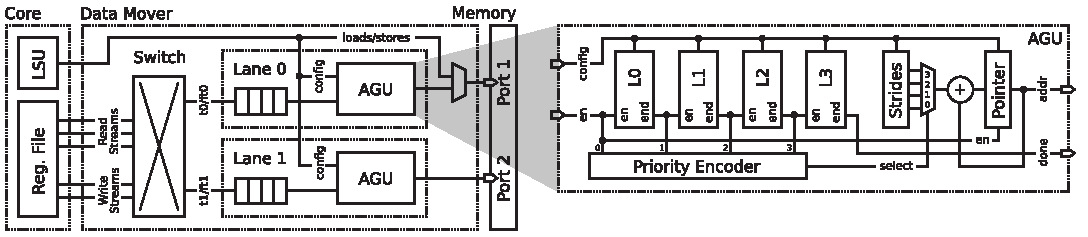
\includegraphics[width=0.87\linewidth]{images/ssr-data_mover.pdf}
 		\caption{Data mover interfaces and inner structure (Left); Internal design of Address Generator Unit (Right) - Figure adapted from \cite{9068465}}
 		\label{fig:ssr-data_mover}
	\end{center} 
\end{figure}

For each processed stream, the AGU is configured in either reading mode, generating memory addresses, or writing mode, producing tags for each datum to be written. It's noteworthy that the processing of streams cannot be interleaved; thus, the same mode has to persists per AGU until the conclusion of the address pattern.


A positive aspect arising from the previously mentioned constraint is the proactive capability of the data mover to perform memory reads using the defined configuration. This behavior facilitates quicker access to data, as whenever the processor decides to read from an SSR, the data is already available. This stands in contrast to normal data accesses, where each request needs to be individually made and awaited.

Unfortunately, due to the design of the data mover and the pro-active read, memory incoherence could occur since a lane could have read a value from memory and placed it in the \textit{FIFO} before the other lane could have updated the same memory location with a new value, for this reason, to avoid data races write operation cannot initiate on a section of memory that has been set to read from.

\subsubsection{Execution Flow}

The execution of a program compiled for this solution starts with the setup of the configuration registers present in the AGUs of the data mover. These registers define the loop dimensions of a stream, allowing for a total of four dimension loops. After the activation of stream semantics in the cores' CSR the iteration of the computations occurs with the AGU loop counters iterating over the preconfigured access patterns and providing the necessary data to the main pipeline of the core.

At the end of the code section optimized for the use of stream semantics, the program executes an instruction to deactivate the use of stream semantics, allowing the core to utilize every register as normal registers.

\subsubsection{Result Analysis}


Several tests were conducted with a focus on evaluating power consumption, performance, efficiency, and the implementation area. In their research, Schuiki \textit{et al.} \cite{9068465} observed a performance increase ranging from 2x to 5x, attributed to the overall reduction in instructions. This improvement was achieved with only a minor increase in the core area (11\%), accompanied by a notable decrease in cache energy consumption by up to 5.6x. These findings substantiate the belief in the potential effectiveness of streaming mechanisms.

While the outcomes achieved for the compiled workloads were favorable, there is room for improvement in the compilation method. The current compiler approach applies SSR indiscriminately to every encountered loop, this leads to the utilization of SSR in smaller loops that do not derive significant benefits, mainly due to the higher setup time required. This observation underscores a potential drawback and emphasizes the necessity for additional research and enhancements.

As also highlighted by Schuiki \textit{et al.} \cite{9068465}, the design of the Address Generator Unit (AGU) in the data mover restricts the applicability and gains of the implementation, primarily due to the limitations in the types of memory access patterns that can be configured. Other research has explored similar principles to those used in SSR but with the capability to accommodate more intricate data patterns, like the Indirection Stream Semantic Register (ISSR) extension \cite{9474230}.



\section{Vector Extensions}

As it was previously discussed, enhancing data load and store operations contributes to the improvement of the system's memory access latency and overall performance. However, individual computations on this data still occur sequentially. This is where vector extensions prove beneficial. Vector extensions employ Single Instruction, Multiple Data (SIMD) instructions across a vector of data in a single execution step, enabling increased system throughput.


\subsection{ARM Scalable Vector Extention}
\label{label:arm-sve}

The ARM approach to a vector-length-agnostic programming model was the definition of ARM SVE \cite{arm-paper}. SVE brings a new architectural state with the inclusion of:
\begin{itemize}
    \item 32 new scalable vector registers, \textit{Z0 to Z31}, with a total width ranging from 128 to 2,048 bits depending on the implementation;
    \item 32 128-bit wide Advance SIMD registers, \textit{V0 to V31}, allowing for 64-, 32-, 16- and 8-bit scalable containers
    \item 16 scalable predicate registers \textit{P0 to P15} and a set of control registers \textit{ZCR\_EL1 to ZCR\_EL3}.
\end{itemize}


\subsubsection{Predication}
The ARM SVE solution allows programmers to think at a higher level of abstraction regarding vector length. This is possible through predicate registers that dynamically modify the vector length during execution. This technique allows the computation of only those lanes that matter, as opposed to the usual SIMD strategy of computing the whole vector and discarding unwanted values through masking.

\begin{figure}[H]
	\begin{center}
 		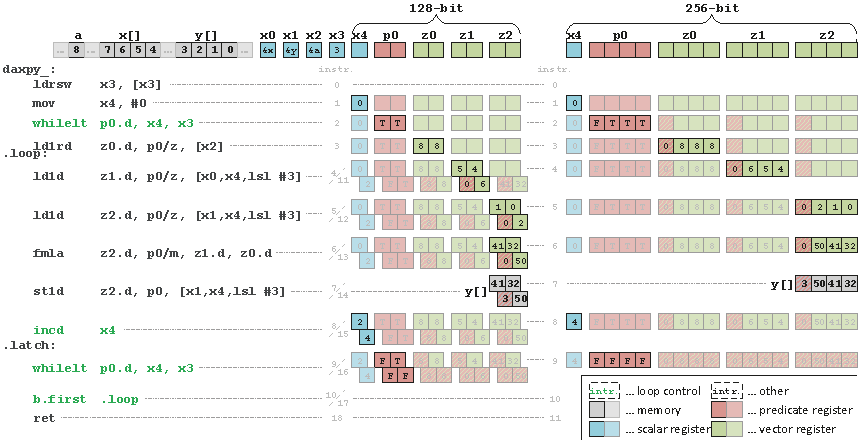
\includegraphics[width=0.77\linewidth]{images/predicator-example.pdf}
 		\caption{Cycle by cycle example of daxpy with n = 3 and hardware vector lengths of 128- and 256-bit - Figure from \cite{arm-paper}}
 		\label{fig:arm-sve-assembly}
	\end{center} 
\end{figure}

Figure \ref{fig:arm-sve-assembly} illustrates a step-by-step example of a Daxpy program for a vector length of 128 and 256 bits. The use of a predicate variable is demonstrated in the 128-bit configuration, with both its values set to true on the first comparison, utilizing the full dimension of the vector. This state of the predicate signifies that the load and computation of values occur in both positions of the variables \textit{z0, z1, z2}. After the loop iteration,  the variable tracking the number of processed elements is incremented (in this case, by the total number of float elements in the vector), and compared with the total number of values to be processed. From this comparison, another predicate is generated, and, since two elements have been processed and the total is three, the new predicate indicates the execution of instructions over only a single entry of \textit{z0, z1, z2} in the next iteration.

Something similar happens in the 256-bit vector configuration. However, the initial comparison generates a predicate with the last position being false. This means the vector won't be utilized in full, and the next predicated instructions to execute should only compute three values.

SVE also includes in its extended instruction set a family of \textit{while} instructions that operate by populating a new predicate through the use of a scalar counter. The value of this stride can be incremented not only by the value of the total number of elements in the system vector but also through more complex increment functions like incrementing by the number of active lanes, or the largest multiple of a data element on a vector, allowing for a powerful data access and manipulation. 

Due to this nature of vector-length-agnostic programming, situations that require vector initialization can become more difficult. To address this complexity, the SVE extension incorporates a set of instructions capable of dynamically generating vector initialization during runtime. This dynamic approach is particularly useful as it adapts to pattern initializations, allowing for flexibility and efficiency in vector initialization processes.

Some examples of specific vector initialization are as follows:
\begin{itemize}
    \item Initializing a vector with a set of indexes that start on 1 and increment by 4 can be achieved using \textit{INDEX Zd.S, \#1, \#4} resulting in \textbf{Zd = [1, 5, 9, 13, 17, 21, 25, 29]} for a vector size of 8 elements.
    \item Initializing a predicate vector that is supposed to contain as many triples of the true value as will fit in the vector:\textit{PTRUE Pd.S, MUL3} will result in  \textbf{Pd = [(T,T,T), (T,T,T), F, F]} for a vector size of 8 elements.
\end{itemize}

\subsubsection{Horizontal Reductions}

Another implemented feature in ARM SVE is the ability to do operations across lanes of a vector, essentially taking an operation and applying it to every element of the vector, for example, a sum, a bitwise-and, etc. 

Designing a program with these intrinsics in mind allows for better performance. Fig. \ref{fig:horizontal-reductions} shows a comparison between a simple sum of a multiplication of two vectors. In ARM SVE version without intrinsics (Fig. \ref{fig:horizontal-reductions}.C) the compiler only manages to exploit the vertical multiplication of vectors $a$ and $b$. In the intrinsic version (Fig. \ref{fig:horizontal-reductions}.D) a third vector was created to assist the partial sum during each iteration, leaving the reduction of every element for outside the loop with \textit{faddv}.

\begin{figure}[H]
	\begin{center}
 		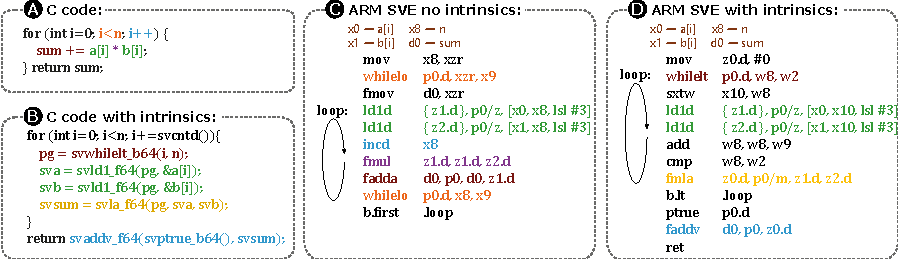
\includegraphics[width=\linewidth]{images/horizontal-reductions.pdf}
 		\caption{Comparison of assembly code between ARM SVE without and with horizontal intrinsics}
 		\label{fig:horizontal-reductions}
	\end{center} 
\end{figure}

\subsubsection{Handling unknown data vector size}


In earlier instances of ARM SVE examples, predicates have consistently played a crucial role in the loading, storing, and manipulation of data. Nevertheless, scenarios may arise where determining the size of the vector becomes impractical before the data load. 

One approach in such situations could be to load as much data as can be fitted into a vector. However, this approach introduces the risk of loading invalid or protected values from memory, potentially triggering a fault.

To avoid the aforementioned problem, speculative vectorization can be utilized. SVE incorporates a distinctive predicate that is generated when employing a memory-probing instruction. This instruction essentially examines the memory entries, starting at a base address, and return a predicate that indicates the regions in memory corresponding to the desired data.

This feature allows for uncounted loops with break conditions to be still manipulated in vectorization form, without the need for size specification. Figure \ref{fig:ffr-example} depicts the utilization of FFR in an uncounted loop on a machine with a vector length set to four and a total data size of six. In the initial iteration, the returned predicate encompasses all entries marked as true, facilitating the loading of a total of four elements. Subsequently, in the second iteration, only the first two elements are identified as true, allowing the program to proceed by loading two values. As the loop progresses to the third iteration, the predicate indicates that no more data is available beyond that point, enabling the program to continue without further loop iterations.

\begin{figure}[H]
	\begin{center}
 		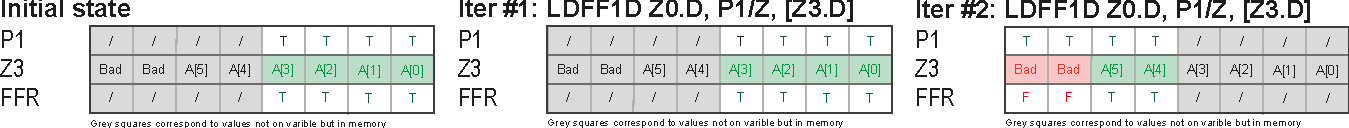
\includegraphics[width=\linewidth]{images/ffr-example copy.pdf}
 		\caption{Simplified example of loop iteration and vector partition with FFR}
 		\label{fig:ffr-example}
	\end{center} 
\end{figure}

Nevertheless, while this feature effectively addresses the challenge posed by an unknown data size, it introduces a potential downside. The increase in the number of instructions within the loop may contribute to heightened pressure on the processor pipeline. This, in turn, could impact the overall efficiency of the vectorization process. Balancing the advantages of dynamic size handling with the potential impact on pipeline performance becomes a crucial consideration in optimizing the execution of SVE instructions.

\subsubsection{Result Analysis}

 The authors of the ARM SVE \cite{arm-paper} conducted a series of workloads in 4 different configurations of the same generic medium-sized out-of-order microprocessor, one without the implementation of SVE, and three implementations with SVE and where the vector size was changed to 128-, 256- or 512-bit vector length.
The overall results of the SVE implementations showed significant speedups, with workloads achieving 3x, 5x and 7.5 for the SVE 128-bit, the SVE 256-bit, and  SVE 512-bit implementation, respectively, when compared with the non-SVE implementation. Some workload tests presented no speedup due to the nature of the test since they do not benefit from vectorization, so performance was very similar between the four configurations.



\subsection{RISC-V Vector Extention (RVV)}
\label{label:rvv}

Just like the ARM Scalable Vector Extension (SVE), the \acrfull{RVV} adopts an \acrfull{ISA} that centers around a vector-length-agnostic programming model. \acrshort{RVV} operations distinguish themselves solely based on vector-vector and vector-scalar distinctions, considering signed and unsigned types, without specifying element lengths. Consequently, the element length becomes a dynamic parameter in this context. Moreover, \acrshort{RVV} allows the utilization of only a segment of a vector register or even a combination of multiple vector registers, introducing the necessity for dynamic parameters in such scenarios.




\subsection{Unlimited Vector Extention with Data Streaming Support}
\label{label:uve}

%Unlimited Vector Extention is a novelty solution that aims to surpass the existing problems of current state-of-the-art solutions of scalable vector extensions through the use of a data streaming engine, combining streaming and SIMD processing, which allows the exploitation of data parallelism.


%The proposed ISA tries to reduce latencies associated with loop control, memory access indexing, and memory access by using new instructions that allow a pre-configuration of the stream and the memory access patterns. 
%This anticipation of the access control allows for accurate and fast prefetching even with multidimensional arrays or indirect memory accesses. 


The \acrfull{UVE} \cite{uve-paper} represents a novel solution designed to combine faster data access with increased system throughput. Achieving this objective involves the incorporation of a data streaming engine that seamlessly integrates streaming and SIMD processing, thereby enabling the effective utilization of data parallelism.

The envisioned \acrshort{ISA} strives to mitigate latencies commonly associated with loop control, memory access indexing, and memory access. This is achieved by introducing novel instructions that facilitate the pre-configuration of the data stream and memory access patterns. The innovative feature of reconfiguration of access control enables precise and expedited prefetching, even when dealing with multidimensional arrays or indirect memory accesses.


\subsubsection{UVE Features}

\begin{figure}[H]
    \centering
    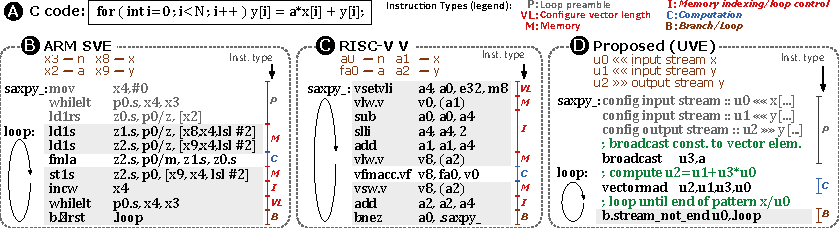
\includegraphics[width=\linewidth]{images/UVE-Comparison.pdf}
    \caption{Assembly code comparison between ARM SVE, RVV, and UVE - Figure from \cite{uve-paper}}
    \label{fig:uve-comparison}
\end{figure}

The main difference of this solution from other recently developed SIMD solutions (ARM SVE and RISC-V Vector extension (RVV)) comes from features like:
\begin{itemize}
\item[]  \Tbullet{F1}{Decoupled Memory Access} The ability to decouple the memory accesses from the computation part by streaming the data directly to the register, allowing the occurrence of loads/stores in parallel with the data manipulation, thus reducing the memory access latency.


\item[]  \Tbullet{F2}{Indexing-free Loops} By describing the load/store patterns in advance, it allows minimizing the number of instructions related to memory indexing, reducing the pressure on the processor pipeline (see Fig.\ref{fig:uve-comparison}.D). 



\item[]  \Tbullet{F3}{Simplified Vectorization} The use of memory access pattern descriptors allows the Streaming Engine to anticipate all non-coalesced accesses as linear patterns and deliver them to the processing unit. This leads to a simplified vectorization since memory is always aligned from the execution pipeline point of view - see Fig. \ref{fig:uve-mem-access}. 


\item[]  \Tbullet{F4}{Implicit Load/Store} Since the streams are described in the loop preamble, the indexing instructions can be removed, meaning that all explicit loads and stores are associated with active streams and different vector registers.
\end{itemize}

Besides the mentioned features, UVE is also register-size agnostic, similar to SVE and RVV. However, in UVE, there is no need for size control instruction since the Streaming Engine automatically disables all vector elements that fall out of bounds, making the loops simpler with a minimal set of control functions.


\begin{figure}[H]
	\begin{center}
 		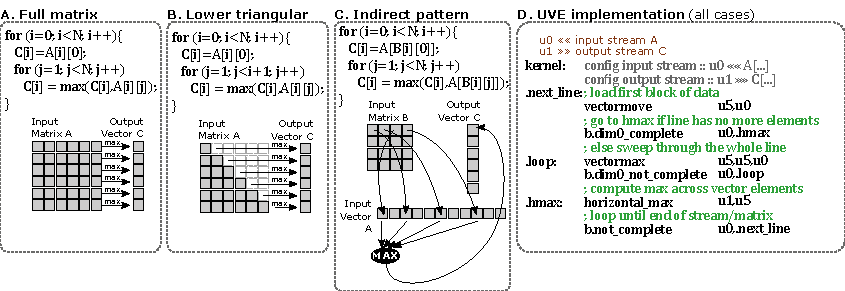
\includegraphics[width=\linewidth]{images/UVE-pseudo-code.pdf}
 		\caption{UVE pseudo-code implementation for the computation of the maximum
across the rows on three possible matrices: (A) full matrix, (B) lower triangular
matrix, and (C) full matrix with pointers to an array - Figure adapted from \cite{uve-paper}}
 		\label{fig:uve-mem-access}
	\end{center} 
\end{figure}


\subsubsection{Microarchiteture Extension}

In order to decouple the memory accesses the \acrshort{UVE} implementation proposed by, Domingos \textit{et al.} \cite{uve-paper} assumed the incorporation of a streaming engine in the microarchitecture of a CPU core. Adding such a feature requires the modification of other preexisting components, like the instruction decoder (to support SIMD operations as well as the streams configuration, control, and manipulation instructions)  modifying the reorder buffer to enable the renaming of vector registers and streams, allowing for speculative stream configuration, and lastly, add a new execution unit on the execution stage to process all the stream manipulating instructions. The proposed changes and their placement can be seen in Fig. \ref{fig:uve-arch}.

\begin{figure}[H]
	\begin{center}
 		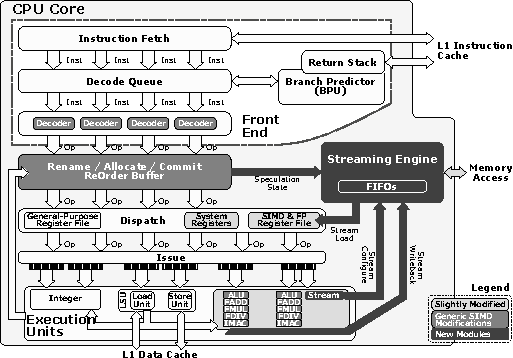
\includegraphics[width=0.67\linewidth]{images/UVE-arch.pdf}
 		\caption{Modifications overview for UVE support}
 		\label{fig:uve-arch}
	\end{center} 
\end{figure}

The implemented streaming engine has the responsibility of managing all the input and output streams. Its inner structure is depicted in Figure \ref{fig:uve-engine} and is composed of 4 main modules: the \acrfull{SCROB} (unit corresponding to the sorting queue and validation on the left of Figure \ref{fig:uve-engine}), a stream table, a stream scheduler and address generator, and a set of load/store FIFO queues.

\begin{figure}[H]
	\begin{center}
 		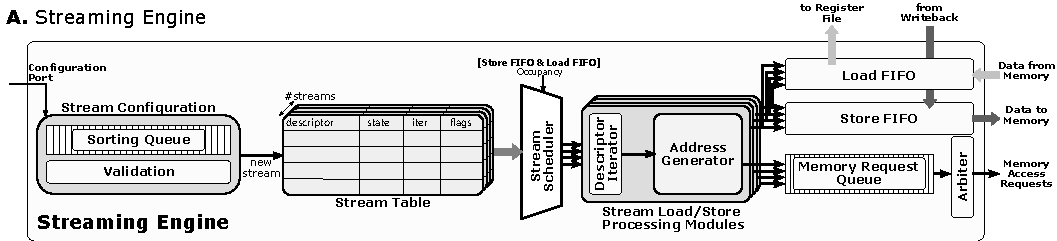
\includegraphics[width=0.97\linewidth]{images/uve-engine.pdf}
 		\caption{Streaming engine structure}
 		\label{fig:uve-engine}
	\end{center} 
\end{figure}


The Stream processing starts with the configuration of the streams. Whenever a configuration instruction reaches the rename stage of the pipeline, it is moved to the first unit of the streaming engine, the stream configuration queue, where it will wait until all operands of the configuration descriptor are available. This approach of using a dedicated buffer unit is used since complex access patterns might require multiple instruction and holding such instructions on the pipeline commit buffer would prevent the speculative configuration of streams, impacting performance. Following the validation of the configuration, the configured stream is moved to the stream table, allowing the stream scheduler to start processing the stream by either pre-loading data for inputs (storing these requests in the memory requests queue and data on the Load FIFO) or calculating addresses for outputs (storing the generated addresses into the Store FIFO). 

The iteration of the chosen streams occurs at each clock cycle and is decided through prioritization of lower FIFO occupancy, by the stream scheduler. Each stream processing model receives a stream and processes it according to their descriptor configuration values, iterating a single dimension and corresponding modifier at a time (this allows for a lower hardware complexity and size).  On each iteration, an update is made to the stream table, keeping the table entries synchronized with the stage of each processed stream. 


\subsubsection{Data Streaming Descriptors}

As mentioned in the previous section, the configuration of streams is encoded in a descriptor-based representation. These descriptors provide the necessary values/parameters utilized on the proposed address modeling equation, defined by Eq. \ref{eq:mem_model}. 

\begin{equation}
    y(X) = y_{\text{base}} + \sum_{k=0}^{\text{dim}_y} x_k \times S_k
    \quad \text{with } X = \{x_0, \ldots, x_{\text{dim}_y}\} \text{ and } x_k \in [O_k, E_k+O_k]
    \label{eq:mem_model}
\end{equation}

Stream descriptors can be classified into two types: \textit{Base Stream Descriptor} and \textit{Descriptor Modifiers}.

\textbf{Base Stream Descriptors} define a uni-dimensional access pattern. It is represented by three-parameters $\{O, E, S\}$ corresponding to the offset $(O_k)$, the size $(E_k)$ and the stride $(S_k)$. These patterns configure the base address of the memory access through the offset value $(O_k)$, the total size of the stream to be loaded/stored with $(E_k)$, and the value of the interleaving space between memory accesses with $(S_k)$. Examples of simple patterns supported by descriptors of this type can be seen in Figs. \ref{fig:stream-descriptors}.B1, B2 and B3.

\textbf{Static Descriptors Modifiers} are descriptors that can be used in conjunction with parameters of Base Stream Descriptors to modify the access pattern, allowing for loop-conditioned accesses, like, for example, a lower triangular memory access as depicted in Fig. \ref{fig:stream-descriptors}.B4. This descriptor is represented as the tuple ${T, B, D, E}$ where $T$ corresponds to the target parameter to modify, $B$ is the modification operator (add or sub), $D$ the value applied with the operator, $E$ the number of times the modifier is applied 

The \textbf{Indirect Descriptor Modifier} allows for the content of a stream to modify the values of another stream, creating indirect and indexed scatter-gather patterns. This modifier is represented by the tuple ${T, B, P}$, with $T$ being the target parameter, $B$ the behavior parameter (supporting adding a dynamic displacement, subtracting a dynamic displacement, and setting a value directly) and $P$ corresponding to the pointer of the origin data stream. Fig. \ref{fig:stream-descriptors}.B5 shows the use of this description in order to create indirect memory access on data of vector $B$ by indexing it from values of vector $A$

As depicted by Fig. \ref{fig:stream-descriptors}.A1, A2, A3, all three descriptors can be used in multidimensional access patterns as well as in a combination of each other, creating complex memory access patterns.

\begin{figure}[H]
	\begin{center}
 		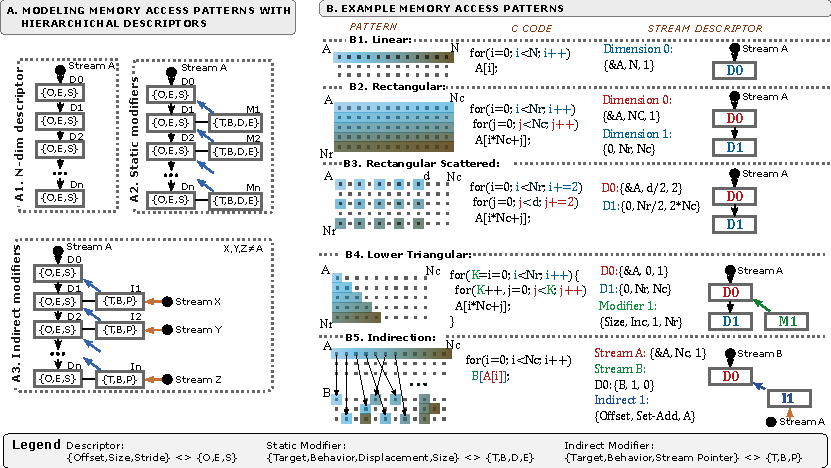
\includegraphics[width=.87\linewidth]{images/UVE-Descriptors.pdf}
 		\caption{Examples of memory access patterns with UVE descriptors - Figure adapted from \cite{uve-paper}}
 		\label{fig:stream-descriptors}
	\end{center} 
\end{figure}



\subsubsection{ISA Extension}
To support the added functionalities of the streaming data structures and the use/manipulation of SIMD vector operations, the ISA needs to be extended with the following type of instruction: 
\begin{itemize}
    \item \textbf{Stream configurations}, as the name implies, these instructions are responsible for encoding the descriptors/modifiers described above, controlling the behavior of the streaming engine. 

    \item \textbf{Stream control} instructions enable the control of streams and allow vector registers to stop/restore momentarily. This behavior control enables the execution of multiple processes without interfering with stream configurations.

    \item \textbf{Predication and masking} allow the control of execution of SIMD operations by disabling selected lanes. The proposed UVE provides instructions for predicate configuration based on comparisons and valid vector register elements.

    \item \textbf{Loop control} is assured through three conditional branch instructions: predicate-based (condition tested on a specific predicate register), end-of-stream (a condition on the end of a stream), and end-of-dimension (a condition on a stream dimension end).

    \item \textbf{Vector manipulation} instructions allow the common arithmetic, logic, and shift operations to be applied to the vector registers.
\end{itemize}


\subsubsection{Experimental Results}

All workload tests were conducted using a CPU simulation modeled after an ARM Cortex A76. The result analysis involved comparing the UVE streaming engine implementation with two ARM cores: one featuring only the ARM NEON Extension and the other supporting the ARM SVE.

The overall performance results demonstrated a significant advantage of 2.4x over the ARM SVE. The UVE's speedup was attributed to the reduction in compiled code and the streaming infrastructure, which effectively decreased load-to-use latency and enhanced memory utilization.

\section{Discussion}
The presented overview of the state-of-the-art showcases the existing potential to obtain relevant performance gains through the mutual exploitation of the data streaming and vector processing in RISC-V processor architectures. In particular, the outcomes from the presented proof-of-concept implementation of UVE with Data Streaming Support underscore the need for a thorough hardware description evaluation to validate the potential of this system.

With these considerations in mind, the focal point of this thesis shall be the implementation of the proposed Instruction Set Architecture (ISA) and streaming engine on the 6-stage, single-issue CPU, the CVA6 (as detailed in the subsequent chapter).

The development of such CPU configuration will establish the essential infrastructure for comprehensive testing and evaluation of the system. For instance, it will enable the assessment of performance against alternative hardware implementations of the CPU with streaming and vector manipulation capabilities. Additionally, having this infrastructure in place will facilitate energy consumption and design footprint analyses, allowing for insightful comparisons.





%%%%%%%%%%%%%%%%%%%%%%%%%%%%%%%%%%%%%%%%%%%%%%%%%%%%%%%%%



%% \section{Data Level Paralelism}
%% Most processors currently support \acrshort{DLP} through Single Instructions Multiple Data (\acrshort{SIMD}) operations. \acrshort{SIMD} operations, as the acronym suggests, is the parallel processing of the same instruction with different pieces of data. This parallel processing can lead to higher throughput. In most cases \acrshort{SIMD} is used in program loops that manipulate data collections like arrays, requiring a processor architecture with wide Arithmetic and Logic Units (\acrshort{ALUs}). 
%% 
%% %Although SIMD operations can be seen as something to always use, it has some limitations and can some times be impossible to exploit with certain applications. Executing operations in parallel to different data positions in memory means that said data can not be dependent of each other, the speed gain of parallelizing operations can also be compromised due to memory limitations like memory bandwidth, complex data pattern access and conditional access.
%% 
%% While Single Instructions Multiple Data (\acrshort{SIMD}) operations can be a useful approach to speed up certain applications there are limitations to its use. For example, data being operated in parallel cannot be dependent on each other. Additionally, the speed gain from parallelizing operations can be compromised by memory limitations such as memory bandwidth, complex data pattern accesses, and conditional memory accesses. Therefore, using SIMD operations with certain applications may not always be possible or beneficial.
%% 
%% 
%% Many modern \acrfull{ISA} come equipped with extensions that allow for the use of \acrfull{SIMD} operations. Examples of such extensions are Intel's Advanced Vector eXtension (AVX), the Streaming SIMD Extensions (SSE), and the ARM NEON vector extension\cite{arm-neon}. These extensions utilize special vector registers to distribute the workload of said registers throughout the \acrshort{ALUs}.
%% 
%% 
%% 
%% Some solutions have been developed to overcome this limitation, focusing on vector-length agnostic code and working with variable-length registers.
%% 
%% 




%% ############################################################################
%%  \section{Data-Prefetching}

%%  Despite advancements in making processors faster, slowdowns can occur if the processor has to stall during data retrieval from memory. In such cases, the entire system's efficiency is compromised, highlighting the critical impact of memory access speed on overall performance.
%%  
%%  To address this concern, data prefetching has emerged as a strategy explored through software implementations, hardware implementations, and hybrid solutions that combine both methodologies.
%%  
%%  Prefetching based on differences in memory access sequences can be unreliable in detecting patterns because of aggressive optimizations such as out-of-order execution that can change the order of memory access. Due to this optimization, the sequence of memory addresses used to calculate the difference can be altered, leading to inaccurate predictions.
%%  

%%  \subsection{Complex Access Patterns}
%%  Although memory data access occurs, in a lot of scenarios, in a "linear way", meaning that memory stores with a delta spacing of +1, some workloads can contain repeating multi-delta sequences, making it more difficult to predict and prefetch \cite{7856594}.
%%  
%%  An example of this type of workload is the Lattice Boltzmann Method (LBM), where memory access is made with the following sequence $(A, A-24, A+1, A-23, A+2, A-22, A+3 ...)$ \cite{7856594}. Further analysis of this sequence shows that the multi-delta sequence can be expressed as a multiple single delta sequence like $(-24, +25), (-24, +25)$ with the base address A changing. It can be even more simplified with a pattern of simply two $+1$ deltas starting on address $A$ and the other on address $A-24$.
%%  
%%  To achieve these patterns, a prefetcher would need the ability to track multiple streams within a physical page as well as compare the new access address with multiple prior addresses in a window, comparing $A$ and $A+1$.
%%  
%%  Some prefetchers that implement these features are the access map pattern matching (AMPM) prefetcher and the Variable Lenght Delta Prefetcher (VLDP)\cite{7856594}. Both work by analyzing the physical address of memory instead of using the program counter (PC) with their structures located outside the main core.
%%  
%%  Another very complicated memory access pattern to predict is the indirect memory access of the form $A[B[i]]$.  
%%  
%%  \subsection{Access Map Pattern Matching}
%%  Whenever data access is requested in AMPM, a "map" of hot memory zones is created to build the pattern information of memory access. A fixed size of the address space defines the memory zones. The AMPM prefetcher stores the entries that correspond to each memory access on a memory access map table and maps it to a specific hot zone. On a memory access, the corresponding entry from the memory access map table is sent to the pattern-matching logic. The pattern-matching logic then generates prefetch requests and issues them to the memory subsystem. This behaviour is illustrated in Fig. \ref{fig:AMPM-overview}
%%  
%%  \begin{figure}[H]
%%      \centering
%%      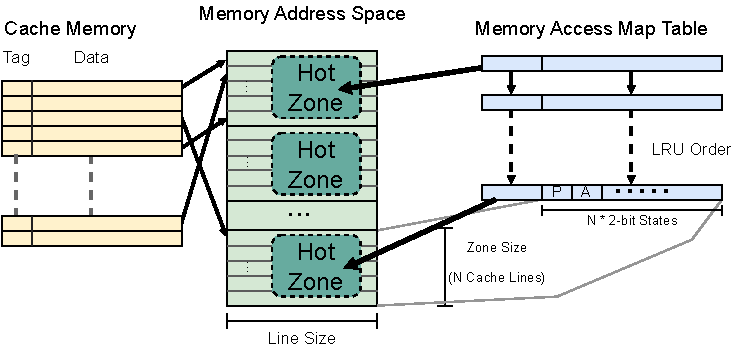
\includegraphics[width=0.77\linewidth]{images/AMPM-Overview.pdf}
%%      \caption{AMPM Structure Overview}
%%      \label{fig:AMPM-overview}
%%  \end{figure}
%%  
%%  Due to the nature of the history of this prefetcher, AMPM does not compute complex data patterns. Since this prefetcher is a most recent access store policy, the predicting capability is limited to simple repeating stride patterns, on top of that the AMPM needs a warm-up period before being able to make accurate predictions. 
%%  
%%  
%%  \subsection{Variable Lenght Delta Predictor (VDLP)}
%%  The VLDP overcomes some of the limitations of AMPM by maintaining a delta history buffer and multiple global delta predictions. The structure shown in Fig. \ref{fig:VLDP-structure} allows VLDP to make complex multi-delta access pattern predictions, which can extend beyond a single memory page. The use of multiple predictions indexed by varying lengths of deltas provides more accurate predictions as the length of the history matches increases.
%%  
%%  
%%  \begin{figure}[H]
%%      \centering
%%      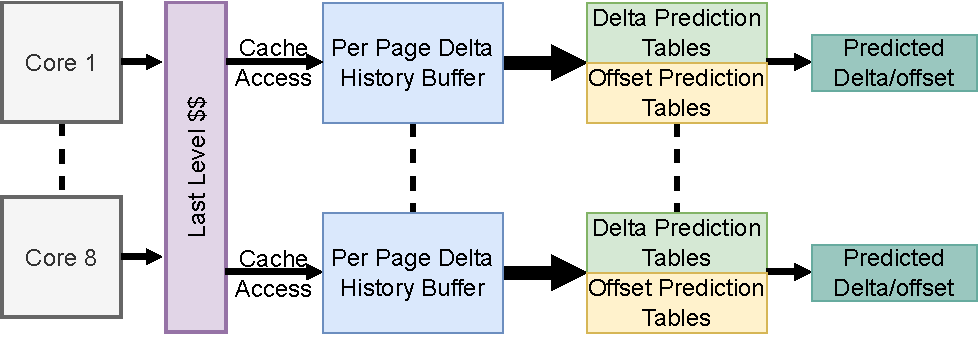
\includegraphics[width=0.77\linewidth]{images/VLDP-overview.pdf}
%%      \caption{VDLP Structure Overview}
%%      \label{fig:VLDP-structure}
%%  \end{figure}
%%  
%%  
%%  Results from \cite{7856594}, shows clear performance improvements of VLDP compared to similar prefetching approaches, achieving a 5.8\% improvement compared to AMPM across a series of test workloads.
%%  
% Data Streaming
% Memory Vectorization